\section{Results}
\label{sec:results}

\subsection{Accuracy relative to the DFT references}
\label{sec:results_fit}

We assess accuracy relative to the DFT references using common held-out geometries for all three functionals.
The test design contains 50 configurations: 25 liquids and 25 structures from hcp-, bcc-, and $\gamma$-TiAl-based solid-solution pools.
Figure~\ref{fig:test_parity} and Table~\ref{tab:fit} compare the fine-tuned models with their corresponding DFT references and with one unchanged pretrained DPA4-Neo baseline.

\input{sections/testset_metrics_table}

\begin{figure*}[t]
\includegraphics[width=\textwidth]{figures/testset_parity.pdf}
\caption{Parity plots for 49 common geometries from the 50-configuration test design. Panels (a)--(c) compare raw energies per atom and (d)--(f) Cartesian force components against PBE, PBEsol, and \rscan{}, respectively. Blue denotes the fine-tuned model; orange denotes the unchanged pretrained model, with open energy symbols. Marker shapes identify liquid (circles), hcp (squares), bcc (triangles), and $\gamma$-TiAl (diamonds) source families. Force statistics contain 34\,446 components. No energy-reference offsets are fitted or applied.}
\label{fig:test_parity}
\end{figure*}

The fine-tuned energy MAEs are 1.11, 1.48, 1.35~meV/atom for PBE, PBEsol, and \rscan{}, respectively; the corresponding RMSEs are 1.47, 1.77, 1.58~meV/atom.
Descriptive 95\% structure-bootstrap intervals for these RMSEs are 1.1176--1.8233, 1.4684--2.0435, 1.3654--1.7743~meV/atom.
PBE has a mean energy residual of $+0.66$~meV/atom and a largest absolute residual of 4.42~meV/atom.
Its energy MAE and RMSE are both smaller than the pretrained values of 2.49 and 2.93~meV/atom.

Fine-tuned force-component RMSEs are 0.0626, 0.0622, 0.0714~eV/\AA, compared with 0.0735, 0.0832, 0.1038~eV/\AA{} for the pretrained model against PBE, PBEsol, and \rscan{}, respectively.
The central values decrease by approximately 15\%, 25\%, 31\% after fine-tuning.
The force-RMSE bootstrap intervals are 0.0582--0.0669, 0.0578--0.0665, 0.0661--0.0765~eV/\AA; their overlap cautions against a strong ranking of the three fits.
Stress RMSEs are 0.072, 0.070, 0.073~GPa.
These pooled Cartesian-component errors differ from the force-vector quantities printed in the training logs.

Raw pretrained energy RMSEs are approximately 427~meV/atom against PBEsol and 4254~meV/atom against \rscan{}.
They include differences in elemental energy references and exchange-correlation descriptions, and therefore do not measure configuration-dependent errors alone.
Force and stress comparisons provide complementary evidence because constant elemental energy shifts leave these derivatives unchanged.

\subsection{Lattice dynamics and thermal density of Ti}
\label{sec:results_crystal}

Figure~\ref{fig:phonons} compares the harmonic response of $\alpha$-Ti at two levels.
The left column shows direct DFT and corresponding fine-tuned DPA4 dispersions against experiment; the right column compares their DOS.
Because the two calculations within each functional use the same DFT-relaxed geometry and phonon protocol, DFT--experiment discrepancies can be assessed separately from the additional DPA4--DFT mismatch.
All six spectra have no frequencies below $-10^{-3}$~THz on the sampled path or phonon mesh, consistent with harmonic stability within this sampling.

The direct DFT curves show that the functional ranking depends on the branch and wave vector.
Near $\Gamma$, the experimental optical features lie at approximately 4.1 and 5.5~THz.
PBE gives an optical doublet at 3.964~THz and a nondegenerate mode at 5.408~THz, closer to these features than the corresponding PBEsol values of 3.786 and 5.758~THz or the \rscan{} values of 4.587 and 5.189~THz.
The higher \rscan{} optical branches around K also lie above the experimental points near 7~THz.
These discrepancies are already present in the direct electronic-structure calculations and therefore cannot be attributed to fine-tuning.
The direct comparison does not support a uniform improvement of the experimental dispersion on replacing a GGA with \rscan{}.
This is a comparison of static harmonic predictions with room-temperature measurements; it is not a separation of exchange-correlation error from thermal and numerical effects.

\begin{figure*}[t]
\includegraphics[width=\textwidth]{figures/phonons_alpha_ti.pdf}
\caption{Harmonic dispersions (left) and densities of states (right) of $\alpha$-Ti: PBE (a,b), PBEsol (c,d), and \rscan{} (e,f). Black points are the same 77 digitized room-temperature measurements reproduced in Ref.~\onlinecite{Souvatzis2007}, attributed there to Stassis \textit{et al.} Blue dashed curves denote direct DFT; orange solid curves denote the corresponding DPA4-finetuned model. Each pair uses the same functional-specific DFT-relaxed cell, $4\times4\times3$ supercell, $\pm0.01$~\AA{} displacements, and Phonopy processing. DOS curves use a $\Gamma$-centered $50^3$ mesh and $\sigma=0.05$~THz broadening, with three modes per atom. The calculations use the numerical settings in Sec.~\ref{sec:phonons}; DFT convergence tests remain pending.}
\label{fig:phonons}
\end{figure*}

The DPA4 curves broadly reproduce the DFT dispersion shapes, but leave systematic optical-mode errors.
The nondegenerate optical frequency at $\Gamma$ decreases from 5.408 to 4.903~THz for PBE, from 5.758 to 4.954~THz for PBEsol, and from 5.189 to 4.221~THz for \rscan{}.
The last change reverses its ordering relative to the optical doublet, which remains close to DFT (4.563 versus 4.587~THz).
Thus, the rearrangement of the \rscan{} optical modes in the fine-tuned model is mainly a representation error of that nondegenerate mode, rather than an intrinsic prediction of the reference functional.
The root-mean-square DPA4--DFT differences of frequency-ordered eigenvalues along the plotted path are 0.209, 0.278, and 0.259~THz for PBE, PBEsol, and \rscan{}, respectively.
These are descriptive spectral discrepancies at the sampled wave vectors, without polarization tracking through crossings; they are not errors relative to experiment.

The DOS panels expose additional differences in the distribution of modes even where the dispersion curves appear close.
For example, the principal PBEsol peak between 7 and 8~THz shifts from 7.194~THz in DFT to 7.328~THz in DPA4, while its height increases from 0.782 to 1.007~modes/(atom\,THz).
The corresponding \rscan{} peak shifts from 7.538 to 7.744~THz.
These changes persist with identical geometry, sampling, broadening, and normalization, and therefore reflect differences in the calculated force constants rather than plotting conventions.
Agreement with experiment alone would not expose all such errors: a model shift can either increase or partially cancel the DFT--experiment discrepancy.

The retained $\alpha_2$-Ti$_3$Al model calculations likewise have no appreciable imaginary frequencies along the sampled $\Gamma$--M--K--$\Gamma$--A--L--H--A path; the largest residual negative magnitude is below $10^{-3}$~THz.
Their maximum frequencies are 9.14, 9.48, and 9.58~THz for PBE, PBEsol, and \rscan{}, respectively.
These results characterize model differences for the compound; the matched DFT/DPA4 and experimental comparisons in Fig.~\ref{fig:phonons} concern elemental $\alpha$-Ti.
Neither the harmonic calculations nor the room-temperature comparison determine the temperature-renormalized phonon spectrum near melting.

The temperature-dependent density of elemental Ti provides a complementary test of the equilibrium volume (Fig.~\ref{fig:density_ti}).
At 300~K, PBE 15k and \rscan{} give similar densities, 4.553 and 4.565~g/cm$^3$, whereas PBEsol gives 4.737~g/cm$^3$; the retained PBE 5k value is 4.559~g/cm$^3$.
The solid-state reference is the tabulation by Zinov'ev,\cite{Zinoviev1989} obtained from thermal-expansion data and the room-temperature density.
Relative to its 300~K value of 4.50~g/cm$^3$, the deviations are approximately $+1.2\%$, $+1.5\%$, and $+5.3\%$ for PBE 15k, \rscan{}, and PBEsol, respectively.
The higher PBEsol density persists over the temperature range considered.
The crystalline branches were obtained from separately prepared $\alpha$-Ti and $\beta$-Ti cells at 300--1100 and 1200--1900~K, respectively, rather than by heating a single crystal through the $\alpha$--$\beta$ transition.
Figure~\ref{fig:density_ti}(a) marks the experimental transition temperatures, approximately 1155~K for $\alpha$--$\beta$ and 1943~K for melting, as reference guides rather than predictions of the models.
The two crystalline phases have very similar densities: the solid-state tabulation gives 4.37 and 4.38~g/cm$^3$ for $\alpha$- and $\beta$-Ti near the transition, a difference of only about 0.2\%.
This small density change is barely visible on the scale of the figure, and the simulated branches likewise show no pronounced discontinuity between the neighboring 1100 and 1200~K points.
The temperature grid does not resolve the transition jump itself.
Within each preparation series the density generally decreases with temperature.
The archived solid-initialized PBE 5k and PBEsol series exhibit a marked decrease between 1600 and 1800~K, while the \rscan{} series retains a higher density at 1800--1900~K.
In the PBE 15k series, the cell initialized as $\beta$-Ti retains crystalline order at 1800~K, with density $4.3632\pm0.0011$~g/cm$^3$, but melts during equilibration at 1900~K, giving $4.2753\pm0.0011$~g/cm$^3$ during liquid production.
Over the last 10~ps, the fraction with $\bar q_6>0.25$ is 0.968 at 1800~K and 0.0004 at 1900~K; the corresponding 10~ps mean-square displacements are 0.77 and 30.30~\AA$^2$.
Persistence of the homogeneous crystal at 1800~K is compatible with metastability above the coexistence melting bracket and does not establish a new equilibrium melting temperature.
This high-temperature decrease is separate from the $\alpha$--$\beta$ transition and motivates the coexistence analysis below, but a density change in a short, initially homogeneous simulation is not itself an equilibrium melting-temperature measurement.

For liquid Ti, we use the experimental reference correlation of Ntonti \textit{et al.},\cite{Ntonti2024}
\begin{equation}
\rho_{\mathrm{ref}}(T)=4.2221-3.952\times10^{-4}(T-1941),
\label{eq:ti_liquid_density_reference}
\end{equation}
where $\rho_{\mathrm{ref}}$ is in g/cm$^3$ and $T$ is in kelvin.
This correlation applies at 0.1~MPa over 1941--3520~K and has a reported expanded uncertainty of 2.0\% at 95\% coverage.
It covers the six liquid temperatures from 2000 to 2500~K without extrapolation; the points at 1873~K lie below its stated range and are not compared with an extrapolated correlation.
Figure~\ref{fig:density_ti}(b) also shows individual liquid-Ti measurements from electromagnetic levitation by Reiplinger and Brillo,\cite{Reiplinger2022} digitized with their reported error bars from the published vector graphic.
These measurements span approximately 1858--2088~K and include undercooled liquid; their experimental error bars are distinct from the expanded uncertainty band of the Ntonti correlation.
The PBE 15k liquid densities are $4.2828\pm0.0008$~g/cm$^3$ at 1873~K and $4.2606\pm0.0011$~g/cm$^3$ at 2000~K, with block standard errors.
The completed PBE 15k recalculations give $4.2415\pm0.0012$, $4.2247\pm0.0011$, $4.2064\pm0.0009$, $4.1899\pm0.0008$, and $4.1717\pm0.0015$~g/cm$^3$ at 2100, 2200, 2300, 2400, and 2500~K, respectively, forming a monotonically decreasing series.
Their mean logged pressures range from 8.11 to 9.71~MPa despite the 0.1~MPa target; the block SEM describes sampling uncertainty and does not include this residual protocol bias.
The PBEsol and \rscan{} liquid branches now use 90~ps production at each temperature, replacing the earlier 30~ps estimates and adding 1873~K.
At 1873~K, the densities are $4.4830\pm0.0006$~g/cm$^3$ for PBEsol and $4.3368\pm0.0007$~g/cm$^3$ for \rscan{}; at 2500~K they are $4.3765\pm0.0008$ and $4.2355\pm0.0007$~g/cm$^3$, respectively.
Both extended series decrease monotonically without fitted smoothing. Diffusion and local-order diagnostics support liquid behavior throughout production, including at 1873~K; this does not determine an equilibrium melting boundary.
Their mean pressures are 7.22--10.47~MPa, with block 95\% intervals excluding the 0.1~MPa target at every point. The density SEM does not include this protocol limitation.
At 2000~K, the reference correlation gives 4.199~g/cm$^3$, compared with 4.261, 4.316, and 4.461~g/cm$^3$ for PBE 15k, \rscan{}, and PBEsol: deviations of $+1.5\%$, $+2.8\%$, and $+6.2\%$.
The 2100--2500~K series decrease less steeply with temperature than the reference; at 2500~K the deviations are $+4.3\%$ for PBE 15k, $+4.4\%$ for PBE 5k, $+5.9\%$ for \rscan{}, and $+9.4\%$ for PBEsol.
PBE remains closest to the central reference in this high-temperature comparison; the PBE 15k value at 2000~K lies within the reference uncertainty band.
The original PBE 5k points remain visible alongside completed 15k calculations. Their difference includes sensitivity to the recording interval and should not be attributed solely to the checkpoint change.
Thus, the liquid-density comparison does not support a uniform advantage of \rscan{} over PBE.
This ordering describes deviations from the central correlation and does not by itself establish statistical separation of the models.

\begin{figure*}[t]
\includegraphics[width=\textwidth]{figures/density_ti_6e45e69b79dc.pdf}
\caption{Temperature-dependent density of elemental Ti compared with experiment. (a) Circles and triangles denote simulations initialized from separately prepared $\alpha$-Ti and $\beta$-Ti cells, respectively; these symbols specify preparation, not persistence of the crystalline phase. The PBE 15k cell initialized as $\beta$-Ti at 1900~K is liquid during production. Vertical lines mark the experimental $\alpha$--$\beta$ transition (approximately 1155~K) and melting (1943~K). Black diamonds are the solid densities in Table~65 of Zinov'ev,\cite{Zinoviev1989} derived from thermal expansion and room-temperature density; dotted lines connect values within each phase. (b) Separately prepared liquids (colored squares). Open black circles and error bars are measurements from Fig.~4 of Reiplinger and Brillo,\cite{Reiplinger2022} digitized from the published graphic, including undercooled liquid. The black line is the Ntonti \textit{et al.}\cite{Ntonti2024} correlation, shown within its stated temperature range; shading is its $\pm2\%$ expanded uncertainty at 95\% coverage. This band is distinct from the measurement error bars and does not describe MLIP uncertainty. Open blue symbols and dashed lines retain all PBE 5k points; filled blue symbols show completed PBE 15k points with block SEM bars. Blue solid segments join adjacent completed temperatures within the same preparation series. PBEsol and \rscan{} in (b) use 90~ps production at 1873~K and 2000--2500~K, sampled every 10~fs, with block SEM bars; their solid-initialized series in (a) are unchanged. Colored solid lines connect sampled means without fitted smoothing. SEM bars exclude protocol and model uncertainties.}
\label{fig:density_ti}
\end{figure*}

\subsection{Solid--liquid coexistence and melting}
\label{sec:results_melting}

The coexistence trajectories provide a clearer distinction between the models.
Figure~\ref{fig:melting} shows the evolution of the solid-like atom fraction near the temperature at which the direction of interface motion changes.
For PBE, the crystal grows at 1750~K and the liquid layer ceases to be resolved at approximately 11~ps.
At 1775~K, both interfaces retreat into the solid, which disappears at approximately 12~ps; the system remains liquid through 100~ps.
The 1800~K trajectory also melts, with the crystalline layer disappearing at approximately 13.5~ps.
Opposite single-phase outcomes therefore give a working bracket of 1750--1775~K.

For PBEsol, crystallization occurs at 1730~K and complete melting at 1770~K.
At 1750~K, the solid fraction fluctuates and decreases overall, but the solid slab survives to the end of the run.
We therefore retain 1730--1770~K as the conservative bracket.
The \rscan{} trajectories yield a narrower observed bracket: the crystal grows in both preparations at 1850~K, whereas the solid layer disappears at 1860~K.
Changing the structural-order threshold or using the bond-correlation criterion preserves the principal distinction between growth and retreat.

\begin{figure*}[t]
\includegraphics[width=\textwidth]{figures/melting_ti.pdf}
\caption{Solid-like fraction in representative 1296-atom Ti coexistence trajectories, using $\bar q_6>0.25$. For PBE, the 1775~K trajectory extends to 100~ps and the 1750/1800~K trajectories to 50~ps. PBEsol and \rscan{} trajectories are 50~ps long; panel time ranges differ accordingly. The two \rscan{} trajectories at 1850~K have different preparation histories; the dashed curve denotes the second preparation. The fraction diagnoses growth or retreat of the crystalline slab, rather than an exact thermodynamic phase fraction.}
\label{fig:melting}
\end{figure*}

\begin{table}[tb]
\caption{Ti melting estimates and brackets from opposite single-phase outcomes. PBE uses 50~ps at 1750~K and 100~ps at 1775~K; the other models use 50~ps trajectories. The PBE estimate is a rounded representative value within its 25~K bracket. The reference value is 1943~K, as used in Ref.~\onlinecite{Wang2012}. Brackets are protocol-dependent observations, not confidence intervals.}
\label{tab:melting}
\begin{ruledtabular}
\begin{tabular}{lrrr}
Model & Estimate (K) & Bracket (K) & Bias (\%)\\
\hline
PBE  & $\sim1760$ & 1750--1775 & $-9.4$\\
PBEsol   & $\sim1750$ & 1730--1770 & $-9.9$\\
\rscan{} & $\sim1855$ & 1850--1860 & $-4.5$\\
\end{tabular}
\end{ruledtabular}
\end{table}

The working estimates are approximately 1760, 1750, and 1855~K for PBE, PBEsol, and \rscan{}, respectively (Table~\ref{tab:melting}).
Relative to 1943~K, the \rscan{} model reduces the underestimation from about 180--190~K to 88~K.
Using 1941~K as the experimental reference would not change this ranking.
The approximately 100~K separation between \rscan{} and the two GGA-based potentials exceeds the widths of their observed brackets.
This makes melting the clearest improvement obtained with \rscan{} in the present set of tests.
The 1850--1860~K bracket must nevertheless not be interpreted as a total uncertainty of $\pm5$~K: finite cell size, interface interactions, preparation dependence, and finite observation time remain unquantified.

\subsection{Liquid density and mixing thermodynamics}
\label{sec:results_thermo}

We next compare properties across composition, using $x_{\mathrm{Al}}=N_{\mathrm{Al}}/(N_{\mathrm{Al}}+N_{\mathrm{Ti}})$ throughout.
At 1873~K, all models predict a monotonic decrease in density as Ti is replaced by Al (Fig.~\ref{fig:liquid_density}).
PBE gives the lowest densities and PBEsol generally the highest, with \rscan{} between them.
The comparison uses the densities tabulated at 1873~K by Brillo \textit{et al.}\cite{Brillo2025}
PBE is closest overall to this reference set.
Using equal weight for each of the 11 common compositions and averaging multiple published entries at the same composition gives mean absolute deviations of 0.112, 0.246, and 0.189~g/cm$^3$ for PBE, PBEsol, and \rscan{}, respectively.
The corresponding mean absolute relative deviations are 3.3\%, 7.5\%, and 5.8\%.
These are descriptive discrepancies against the tabulated values, rather than statistically weighted goodness-of-fit measures.

\begin{figure*}[t]
\includegraphics[width=\textwidth]{figures/liquid_density.pdf}
\caption{Liquid density (a) and excess molar volume (b) at 1873~K. The PBE series uses 30~ps production after 30~ps equilibration; PBEsol and \rscan{} retain their original series. Black symbols in (a) are the printed densities in Table~7 of Ref.~\onlinecite{Brillo2025}; separate entries at the same composition are shown individually. Reference excess volumes in (b) are recomputed from those densities and their pure-component endpoints. Each MLIP excess volume uses its own pure-liquid references. Some experimental reference values represent extrapolated or undercooled-liquid states.}
\label{fig:liquid_density}
\end{figure*}

All three models predict negative excess molar volumes at the sampled interior compositions.
At 1873~K, the discrete minima are approximately $-0.96$~cm$^3$/mol at $x_{\mathrm{Al}}=0.6$ for PBE, $-0.83$~cm$^3$/mol at $x_{\mathrm{Al}}=0.6$ for PBEsol, and $-1.02$~cm$^3$/mol at $x_{\mathrm{Al}}=0.6$ for \rscan{}.
Thus, mixing produces substantial volume contraction relative to each model's pure-liquid reference volumes.
The published densities also imply a pronounced contraction over much of the intermediate and Al-rich composition range, but yield appreciable scatter and positive excess volumes at some Ti-rich compositions.
The models therefore capture the principal contraction without reproducing all features of the reference data.
Absolute density and excess volume probe different combinations of pure-component and alloy errors; agreement in one does not guarantee agreement in the other.

\draftnote{The density comparison currently uses the printed 1873~K column of Table~7 in Ref.~\onlinecite{Brillo2025}. At least one equiatomic entry is inconsistent with its listed temperature-fit coefficients. Resolve the reference convention before finalizing numerical error metrics. Some values are extrapolated, and Ti-rich liquids at 1873~K are below the experimental liquidus.}

The mixing enthalpy gives a different ranking (Fig.~\ref{fig:mixing}).
At 2000~K, all three models predict strongly exothermic mixing and a broad minimum near intermediate composition.
The PBE and PBEsol minima are $-25.0$ and $-25.4$~kJ/mol at $x_{\mathrm{Al}}=0.5$.
The extended 60~ps \rscan{} series gives $-31.66\pm0.19$~kJ/mol at $x_{\mathrm{Al}}=0.5$ and $-31.74\pm0.20$~kJ/mol at 0.6.
Although the latter is the numerical minimum, their difference is only $-0.081\pm0.263$~kJ/mol, including the shared pure-component covariance, so its position is not resolved between these compositions.
The PBE minimum is $-25.01\pm0.30$~kJ/mol.
The quoted errors are propagated block standard errors; the longer \rscan{} sampling changes the mean curve by at most 0.39~kJ/mol and does not uniformly reduce these errors.
The values reported here use the thermodynamic enthalpy at the imposed external pressure, as defined in Sec.~\ref{sec:thermodynamics}, and consistent pure-liquid reference calculations.

The experimental comparison is based on calorimetric points reproduced in Fig.~7 of Witusiewicz \textit{et al.}\cite{Witusiewicz2008}
Their CALPHAD curve is not used as an experimental dataset.
The reproduced points indicate a minimum of approximately $-29.5$ to $-30$~kJ/mol near $x_{\mathrm{Al}}=0.5$--0.6.
PBE and PBEsol underestimate the depth of this minimum, whereas \rscan{} overestimates it.
Across nine digitized interior compositions, the provisional mean absolute deviations are approximately 3.6, 3.1, and 1.5~kJ/mol for PBE, PBEsol, and \rscan{}, respectively.
Consequently, \rscan{} better reproduces the overall composition dependence under this metric, although it is not uniformly closer at every composition.

\begin{figure}[htbp]
\includegraphics[width=\columnwidth]{figures/mixing_enthalpy.pdf}
\caption{Liquid mixing enthalpy at 2000~K compared with calorimetric points reproduced in Ref.~\onlinecite{Witusiewicz2008}. Reference points are a provisional digitization of calorimetric symbols. PBE error bars propagate the maximum block SEM over 3, 5, and 6~ps blocks; PBEsol uses six 5~ps blocks and \rscan{} uses twelve 5~ps blocks from 60~ps production. Both pure-liquid references are included. These are diagnostic standard errors, not final confidence intervals. Lines connect sampled compositions.}
\label{fig:mixing}
\end{figure}

These results quantify a difference in the energetic preference for the alloy relative to its pure liquids.
They do not, by themselves, identify a particular electronic mechanism or establish chemical short-range order.

\draftnote{The original calorimetric reports behind Ref.~\onlinecite{Witusiewicz2008} are unavailable. The current digitization has an estimated reading tolerance of about 0.2~kJ/mol, which is not an experimental uncertainty. Finalize the digitization and trajectory uncertainty analysis before treating the quoted deviations as publication-ready metrics.}

\subsection{Liquid viscosity}
\label{sec:results_viscosity}

Both potentials predict a nonmonotonic composition dependence of liquid viscosity at 1873~K (Fig.~\ref{fig:viscosity}a).
Adding Al initially increases the viscosity, producing a broad maximum at intermediate composition, followed by a pronounced decrease toward the Al-rich end.
The largest sampled values are $5.02\pm0.19$~mPa\,s at $x_{\mathrm{Al}}=0.40$ for PBE and $7.19\pm0.28$~mPa\,s at $x_{\mathrm{Al}}=0.45$ for \rscan{}.
The neighboring compositions have similar viscosities, so neither curve locates a sharp maximum.
The \rscan{} values exceed those of PBE at all eleven sampled compositions.

\begin{figure*}[t]
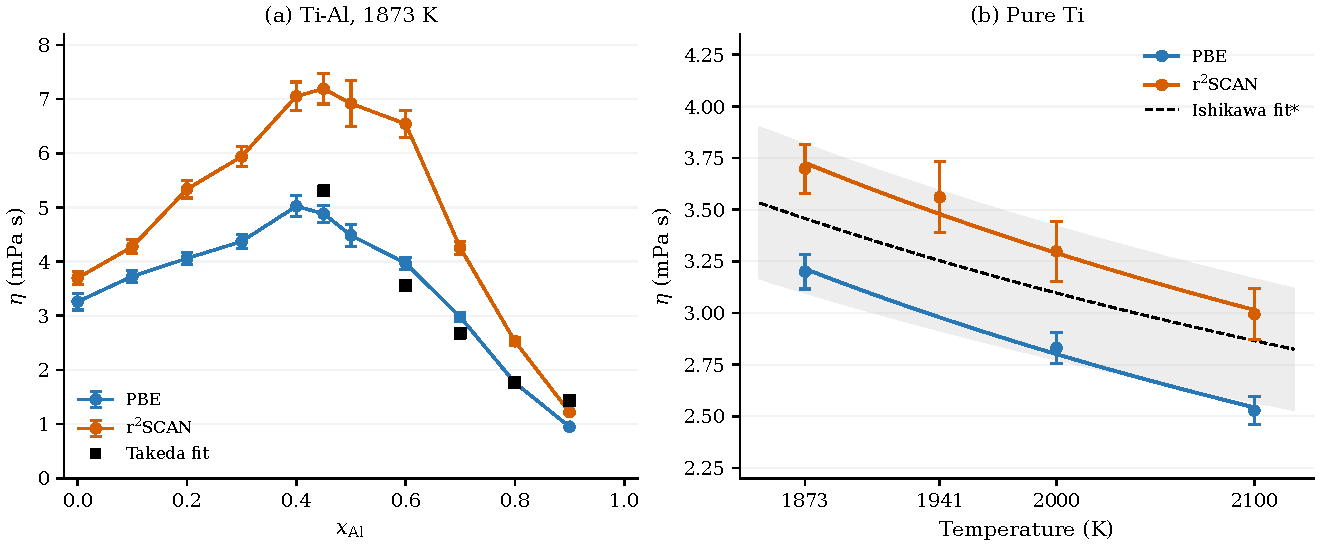
\includegraphics[width=\textwidth]{figures/viscosity.pdf}
\caption{Liquid viscosity versus Al mole fraction at 1873~K (a) and temperature for pure Ti (b). Colored symbols show the PBE and \rscan{} estimates with estimator standard errors. Lines in (a) connect sampled compositions; solid colored curves in (b) are weighted Arrhenius fits. Black squares in (a) are values from the experimental correlations of Takeda \textit{et al.}\cite{Takeda2025} The dashed curve marked with an asterisk in (b) is a provisional transcription of the Ishikawa \textit{et al.}\cite{Ishikawa2012} correlation; the shaded band denotes its reported 10.3\% uncertainty.}
\label{fig:viscosity}
\end{figure*}

PBE is closer to the experimental alloy-viscosity correlations at four of the five compared compositions: $x_{\mathrm{Al}}=0.45$, 0.60, 0.70, and 0.80.
At $x_{\mathrm{Al}}=0.45$, the experimental reference is 5.30~mPa\,s, compared with 4.88 for PBE and 7.19 for \rscan{}.
At $x_{\mathrm{Al}}=0.80$, the corresponding values are 1.764, 1.761, and 2.528~mPa\,s.
The Al-rich state at $x_{\mathrm{Al}}=0.90$ is an exception: \rscan{} gives 1.218~mPa\,s, closer to the reference value of 1.437~mPa\,s than the PBE result of 0.951~mPa\,s.
The two lowest-composition reference values involve a small, 3~K extrapolation of the experimental correlations to 1873~K.
No alloy-viscosity reference is available below $x_{\mathrm{Al}}=0.45$, so the predicted increase on the Ti-rich side cannot be tested by this dataset.

For pure Ti, both potentials predict decreasing viscosity with increasing temperature (Fig.~\ref{fig:viscosity}b).
The PBE estimates decrease from $3.200\pm0.084$~mPa\,s at 1873~K to $2.528\pm0.068$~mPa\,s at 2100~K, while the \rscan{} values decrease from $3.70\pm0.12$ to $2.99\pm0.12$~mPa\,s.
Both series are consistent with smooth Arrhenius temperature dependences within the reported errors.
In particular, the deviations of individual \rscan{} points from the fitted curve do not resolve a change in slope or an anomalous temperature dependence.
Relative to the experimental correlation, PBE and \rscan{} lie on opposite sides at 1873~K, with deviations of approximately $-7.4\%$ and $+7.0\%$, respectively.
At 2000 and 2100~K, \rscan{} is closer to the central experimental correlation.
Thus, the advantage of PBE for most of the compared alloy compositions does not extend uniformly to pure-Ti viscosity over the studied temperature range.

Taken together, the present benchmarks show that the benefit of changing the reference functional depends on the observable.
The \rscan{} potential raises the Ti melting temperature toward experiment and improves the overall mixing-enthalpy comparison, but these gains do not extend uniformly to lattice dynamics, liquid density, or viscosity.
The different rankings are the central outcome of the multi-property assessment and motivate a separate discussion of reference-functional effects, residual fitting errors, and sampling limitations.
